
\chapter{Movimiento circular}
\label{chap:cin1}



% \subsection{Caida libre}
% La observaci\'on experimental, como por ejemplo la caida de una pluma y un bal\'\i n en un tubo de vacio, han establecido que todos los objetos cerca a la tierra se aceleran al la misma tasa constante cuando otros efectos externos est\'an excluidos.


% En un sistema de coordenadas donde la direcci\'on de movimiento es perpendicular a la superficie de la tierra, podemos definir un \emph{vector unitario}, es decir, un vector de magnitud 1 y direcci\'on positiva como $\hat{\mathbf{j}}$, tal que
% \begin{align}
%   |\hat{\mathbf{j}}| = 1,
% \end{align}
% donde los simbolos $|\ |$ representan la magnitud del vector. Entonces el vector de aceleraci\'on gravitacional se puese escribir como
% \begin{align}
%   \mathbf{a}=-g \hat{\mathbf{j}}\,.
% \end{align}

% Los vectores se denotan con letra negrilla o con una flecha arriba $\vec a$. Usaremos la primera opci\'on en este texto. La magnitud del vector de aceleraci\'on gravitacional es entonces:
% \begin{align}
%   |\mathbf{a}|=g=9.8\ \frac{\text{m}}{\text{s}}
% \end{align}

% La soluci\'on a la ecuaci\'on de movimiento
% \begin{align}
%   \frac{d^2y(t)}{dt^2}=-g\,,
% \end{align}

% % ver notas Kowalaski 3-11


\section{Movimiento Circular Uniforme}

Considere el movimiento descrito por la siguiente ecuaci\'on
\begin{align}
  \label{eq:mua}
  \mathbf{r}(t)=r\left(\hat{\mathbf{i}}\cos(\omega t)+\hat{\mathbf{j}}\sin(\omega t)\right),
\end{align}
con $r=\text{constante}$ y $\omega=\text{constante}$, representado en la figura~\ref{fig:mua1}.

La velocidad es
\begin{align}
  \mathbf{v}=&%detalles\\
  r\omega\left(-\hat{\mathbf{i}}\sin(\omega t)+\hat{\mathbf{j}}\cos(\omega t)\right),
\end{align}
representado en la figura~\ref{fig:mua2}. Note que $\mathbf{r}\cdot\mathbf{v}=0$, de modo que los vectores son perpendiculares.

La aceleraci\'on es
\begin{align}
  \mathbf{a}=&%detalles\\
  -r\omega^2\left(\hat{\mathbf{i}}\cos(\omega t)+\hat{\mathbf{j}}\sin(\omega t)\right),
\end{align}
representado en la figura~\ref{fig:mua3}. Note que $\mathbf{a}\cdot\mathbf{v}=0$, de modo que los vectores son perpendiculares. Adem\'as
$\mathbf{r}\cdot\mathbf{a}=-1$, de modo que los vectores son antiparalelos.


\begin{frame}[fragile,allowframebreaks]
  \begin{figure}
    \centering
    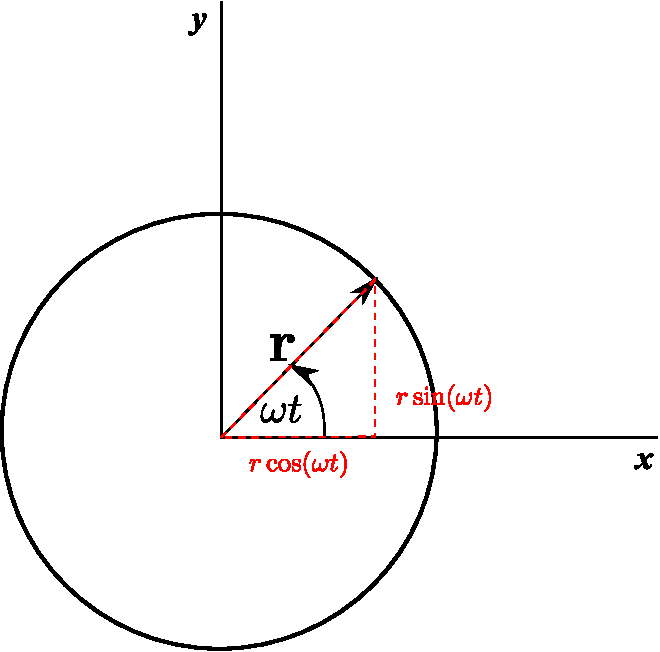
\includegraphics[scale=0.65]{mua1}    
    \caption{Posici\'on}
    \label{fig:mua1}
  \end{figure}

\end{frame}
\begin{frame}[fragile,allowframebreaks]
  \begin{figure}
    \centering
    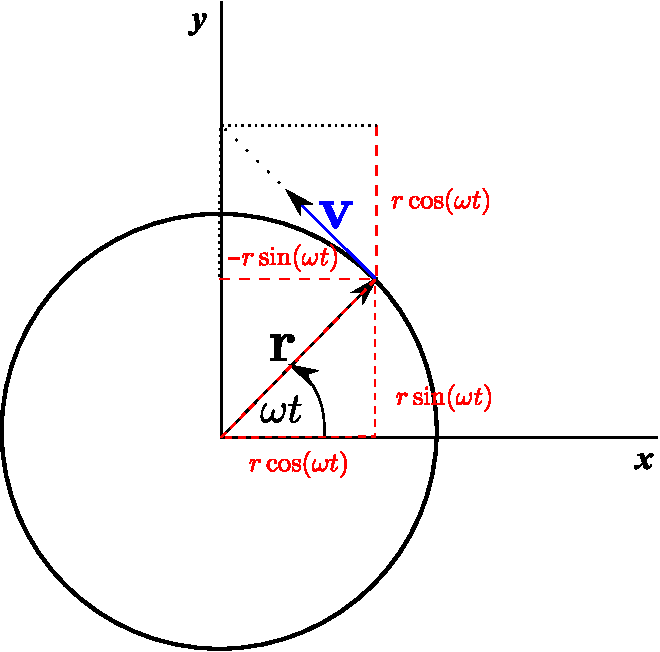
\includegraphics[scale=0.65]{mua2}    
    \caption{Velocidad: tangente a la curva}
    \label{fig:mua2}
  \end{figure}
\end{frame}

\begin{frame}[fragile,allowframebreaks]
  \begin{figure}
    \centering
    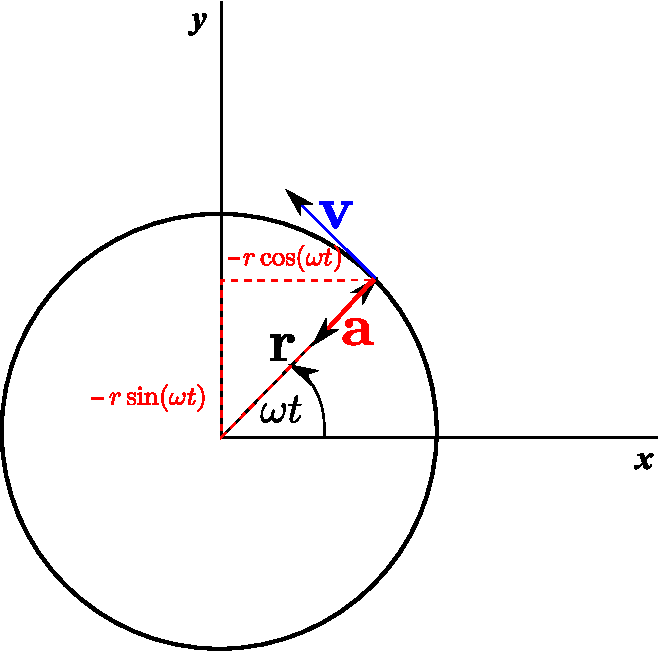
\includegraphics[scale=0.65]{mua3}
    \caption{Aceleraci\'on: centr\'\i peta}
    \label{fig:mua3}
  \end{figure}


\end{frame}

\subsection{Movimiento generalizado en coordenadas polares}
La ecuaci\'on para el vector de posici\'on puede escribirse en general como
\begin{align}
\label{eq:rpol}
  \mathbf{r}(t)=r(t)\left(\hat{\mathbf{i}}\cos[\theta(t)]+\hat{\mathbf{j}}\sin[\theta(t)]\right)\,.
\end{align}
Para algunos problemas es conveniente reescribir \'esta ecauaci\'on en coordenadas polares:
\begin{inprogress}
  Faltan detalles
\end{inprogress}
\begin{align}
  \label{eq:polinv}
  \begin{pmatrix}
    \hat{\mathbf{r}}\\
    \hat{\boldsymbol{\theta}}
  \end{pmatrix}=
  \begin{pmatrix}
    \cos\theta&-\sin\theta\\
    \sin\theta&\cos\theta\\
  \end{pmatrix}
  \begin{pmatrix}
    \;\hat{\mathbf{i}}\;\\
    \hat{\mathbf{j}}\\
  \end{pmatrix}.
\end{align}
con inverso
\begin{align}
  \begin{pmatrix}
    \;\hat{\mathbf{i}}\;\\
    \hat{\mathbf{j}}\\
  \end{pmatrix}=
  \begin{pmatrix}
    \cos\theta&-\sin\theta\\
    \sin\theta&\cos\theta\\
  \end{pmatrix}
  \begin{pmatrix}
    \hat{\mathbf{r}}\\
    \hat{\boldsymbol{\theta}}
  \end{pmatrix}.
\end{align}

La velocidad es
\begin{align}
  \label{eq:vpol}
  \mathbf{v}(t)=&%detalles\\
  \dot{r}(t)\hat{\mathbf{r}}(t)+r(t)\dot{\theta}(t)\hat{\boldsymbol{\theta}}(t)\,.
\end{align}
y la aceleraci\'on es
\begin{align}
\label{eq:apol}
  \mathbf{a}(t)=&%detalles\\
[\underbrace{\ddot{r}(t)}_{{\text{Acel. lineal.}}}
-\underbrace{r(t)\dot{\theta}^2(t)}_{{\text{Acel. centr\'\i peta.}}}]\hat{\mathbf{r}}(t)
+[\underbrace{r(t)\ddot{\theta}(t)}_{{\text{Acel. lineal tangencial.}}}
+\underbrace{2\dot{r}(t)\dot{\theta}(t)}_{{\text{Acel. de coriolis.}}}]\hat{\boldsymbol{\theta}}(t).
\end{align}
\begin{itemize}
\item[\textbf{Ejemplo}] \textbf{MCU}:\\
Comparando (\ref{eq:mua}) con (\ref{eq:rpol}), tenemos para el Movimiento Circular Uniforme que
\begin{align}
  \label{eq:muapol}
   \dot{r}=&0&&&&\\
  \theta(t)=&\omega t\,,&\dot{\theta}(t)=&\omega\,,&\ddot{\theta}(t)=&0\,.
\end{align}
De modo que reemplazando las ecuaciones \eqref{eq:muapol} en las ecuaciones \eqref{eq:vpol}, \eqref{eq:apol}, y usando la transformaci\'on inversa \eqref{eq:polinv}, tenemos que
\begin{align}
  \mathbf{r}(t)=&r\hat{\mathbf{r}}(t)\nonumber\\
  =&r\left(\hat{\mathbf{i}}\cos(\omega t)+\hat{\mathbf{j}}\sin(\omega t)\right),
\end{align}
\begin{align}
    \mathbf{v}(t)=&r\omega\hat{\boldsymbol{\theta}}(t)\nonumber\\
    =&r\omega\left(-\hat{\mathbf{i}}\sin(\omega t)+\hat{\mathbf{j}}\cos(\omega t)\right),
\end{align}
\begin{align}
  \mathbf{a}(t)=&-r\omega^2\hat{\mathbf{r}}(t)\nonumber\\
  =&-r\omega^2\left(\hat{\mathbf{i}}\cos(\omega t)+\hat{\mathbf{j}}\sin(\omega t)\right),
\end{align}
de modo que en el MCU la velocidad no tiene componente radial, y s\'olo
contribuye la aceleraci\'on centr\'\i peta, como era de esperarse.
\end{itemize}

Continuara...

%\left(\right)
%ver inkscape vectores primera capa






%%% Local Variables: 
%%% mode: latex
%%% TeX-master: "mecanica"
%%% End: 

